\chapter{Literature Review}
\label{chapter:background} 

In the following section, I will give overview about Internet of Things (IOT) and Industrial Internet of Things (IIOT), highlighting differences between them. Further, I will describe open issues in IIOT followed by standardization attempts and related work regarding security. At the end of this chapter, I will give a more detailed description of most notable standards, Light Weight Machine-to-Machine (LWM2M) and Web of Things at the end of this chapter followed by Policy Based Communications, which is the basis of this work.

\section{Internet of Things}

%Short introduction about IOT
Internet of things (IOT) is a relatively new concept gaining momentum since the start of this century. Although, first examples
of IOT date back as early as 1983 with an automated inventory system. IOT can be seen as an extension to Internet, with physical devices (such as sensors and actuators) communicating with each other and with humans creating an enormous network.

Nowadays, with the continuous decrease in cost of computational devices, 
we are able to produce powerful devices with communication abilities for a very low price. With the increase in number 
of devices that needs to be connected (some estimates show up to 75 billion connected devices by year 2025\footnote{https://www.statista.com/statistics/471264/iot-number-of-connected-devices-worldwide/}), issues regarding scalability, security, heterogeneity of devices, etc. have emerged. 

These issues are holding back the progress of IOT because it forces companies to create their own proprietary systems to fit their needs, which is only an option for
large companies with financial capabilities to do so. This leads to large number of systems designed for similar purposes but incompatible with each other (due to use of different protocols or architectures). Temporary solution for this problem is to introduce a middle-ware as proposed by \cite{Bandyopadhyay2011} that acts like a bridge between two systems, but this has scalability issues and with the rise of number of connected devices will soon be unacceptable. In order to tackle these issues, several standards have been proposed, most notably smartM2M, oneM2M and most recently LightweightM2M (LWM2M), which will be explained in ~\ref{section:Standardization}. None of these have yet become \emph{de facto} standard.

In the remainder of this section, differences between Industrial Internet of Things (IIOT) and IOT will be introduced followed by open issues of IOT and IIOT  in ~\ref{section:OpenIssues}.


\subsection{Industrial Internet of Things}

In IOT, a rough distinction is made between consumer and industrial IOT according to \cite{Bandyopadhyay2011}. Consumer IOT applications are aimed to make everyday life easier by saving time and money, such as smart locks, smart homes and wearable hearth monitors. On the other hand, industrial IOT (such as production, automation and intelligent computation systems) focuses on how smart machines, data analytics and networked sensors can improve services in business-to-business domain 
\cite{Palattella2016}. As an example, predictive maintenance can generate savings up to 12\% over scheduled repairs, leading to a 30\% reduction in maintenance cost and a 70\% cut in downtime from equipment breakdowns according to Accenture\footnote{https://www.accenture.com/us-en/insight-industrial-internet-of-things}.This usually implies extensive machine-to-machine (M2M) communication compared to consumer IOT, where in most cases real time guarantees are not required.

Generally, IIOT has stricter requirements regarding delay, security and general robustness compared to consumer IOT. This is because failures in these devices can have consequences on safety of people and environment. For example, in a factory setting, pressure sensor installed on an indoor crane can cause serious damage by failing to communicate about an obstruction.

\subsection{Open Issues}
\label{section:OpenIssues}
As previously mentioned, there are many issues surrounding IOT, most notably, lack of standards and security. These issues will be explained in the remainder of the section.

\subsubsection{Standardization}
\label{section:Standardization}

According to Global Standards Collaboration Machine-to-Machine Task Force (GSCM2MTF) there are more than 140 organizations involved in the M2M standardization process worldwide.  
This is a huge vertical fragmentation of IOT market, and it is a result of long history in Industrial use, starting from seventies with process control systems that continued to be used in todays process automation systems. As already mentioned, these systems are proprietary and are incompatible with each other.

In an attempt to resolve this fragmentation issue three notable initiatives stand out. SmartM2M is an initiative led by European Telecommunications Standards Institute (ETSI), it is based on RESTful Service Capability Layer (SCL) \cite{Alaya2014} which is available through open interfaces. Resource tree residing on SCL along with procedures for handling them is standardized following Representational State Transfer (REST) principles allowing technology agnostic way of accessing them. SmartM2M also defines security framework including  authentication, M2M service bootstrap, key agreement and establishment, and M2M service connection procedures, based on a key hierarchy of the M2M node\cite{ETSI1}. Unfortunately, it may have issues with scalability as pointed out by \cite{Grieco2014}, thus, making it unsuitable for IOT and IIOT. 

A follow up project was formed in order to resolve issues with SmartM2M, this time with a broader partnership. It is an international project started by seven telecom standards organizations: Association of Radio Industries and Businesses (ARIB) and Telecommunication Technology Committee (TTC), Japan; the Alliance for Telecommunications Industry Solutions (ATIS) and Telecommunications Industry Association (TIA), United States; the China Communications Standards Association (CCSA), China; the European Telecommunications Standards Institute (ETSI), Europe; and the Telecommunications Technology Association (TTA), Korea. This project is based on RESTfull design, same as SmartM2M, resource naming conventions same as SmartM2M and is grounded on horizontal service layer principle. Although, it relaxes the scalability constraints by using hierarchical organization of different actors in the system. With this improvement with respect to SmartM2M, it is a serious contester to became IOT standard, being already adopted by various companies according to \cite{Park2016}. Along with these improvements, it defines a security architecture in three layers: security functions, security environment abstraction and security environment.

Recently, a new standard has emerged from Open Mobile Alliance (OMA) targeting constrained devices named Light Weight Machine-to-Machine (LWM2M). It defines a fast deployable client-server specification while minimizing memory consumption and network overhead making it very appealing to IOT and IIOT devices. It provides device management and security work-flow for IOT applications in a very light weight manner. Recent results from \cite{Rao2015} show that memory footprint overheads on a client side protocol stack are no more than 6-9\%. 

Another standard has recently been announced by World-wide-web Consortium (W3C) named Web of Things (WOT). This standards aims to provide a middleware (presented as an abstraction layer) to connect different IOT platforms and protocols. Detailed description of LWM2M and WOT will be given in section ~\ref{section:NotableStandards} since they represent two best candidates for this work.


\subsubsection{Security and privacy}
%\fixme{Authentication, Data integrity, Privacy}

Devices in IOT generate, process and exchange vast amount of data that is safety-critical and/or private and they are subject to various attacks. Therefore, it is crucial to assure integrity of the devices code and data from malicious modifications \cite{Control2014}. In IIOT, following two requirements are crucial for security according to \cite{Sadeghi2015}. Availability is most important requirement, because it can lead to loss in productivity and consequently loss of revenue. This is particularly affected by denial of service (DoS) attacks and preventing any system failure that may result in physical damage or harm to humans, particularly affected by sabotage.

There are many security architectures for embedded IOT devices, although, majority of them are too complex for low-end devices. Solutions for low-end devices usually rely on physical (hardware) isolation of security-critical code and data from other software on same device. Examples of such architectures are SMART \cite{Smart}, SPM \cite{SPM}, SANCTUS \cite{Sanctus} and TrustLite \cite{TrustLite} but they all have major flaws. SMART does not allow code changes after deployment. SPM and SANCTUS have hardware assisted task isolation but they are non-interruptible, which violates real-time guarantees. TrustLite requires all software components to be loaded at boot time, which reduces flexibility. TyTAN \cite{Brasser} is the only work that provides secure loading of tasks at runtime, secure inter-process communication, local and remote attestation and real-time guarantees. 
\section{Notable standards}
\label{section:NotableStandards}

Following section will describe two most notable standards which were final candidates for this thesis. These standards come from Open Mobile Alliance and World-wide-web Consortium which are two biggest standardization bodies in mobile communications and Web respectively.

\subsection{Light Weight Machine to Machine (LWM2M)}
\label{section:LWM2M}

OMA has approved first version (V1.0) of LWM2M standard in February 2017, since it is a very recent specification not many implementations exist, although, number has been steadily increasing since then. Most notable implementation by \cite{Rao2015} focuses on client side architecture (residing on IOT devices).

LWM2M provides a light and secure communication interface with compact data model to enable device management and service for IOT (and IIOT) devices. It is a client-server architecture named OMA LWM2M Enabler. Enabler consists of LWM2M Server, which is a central point that takes care of the devices, assigning security keys, registering device capabilities and more. Another part of Enabler is LWM2M Client, which resides on a device and provides necessary information to the Server. Furthermore, it uses Constrained Application Protocol (COAP), instead of HTTP, which has a greatly reduced communication overhead making it ideal for constrained devices (or devices benefiting from efficient communication, as the case in IIOT) along with UDP/SMS transport bindings. Architecture of LWM2M is shown on Figure ~\ref{fig:LWM2MArchitecture}.

\begin{figure}[ht]
	\begin{center}
		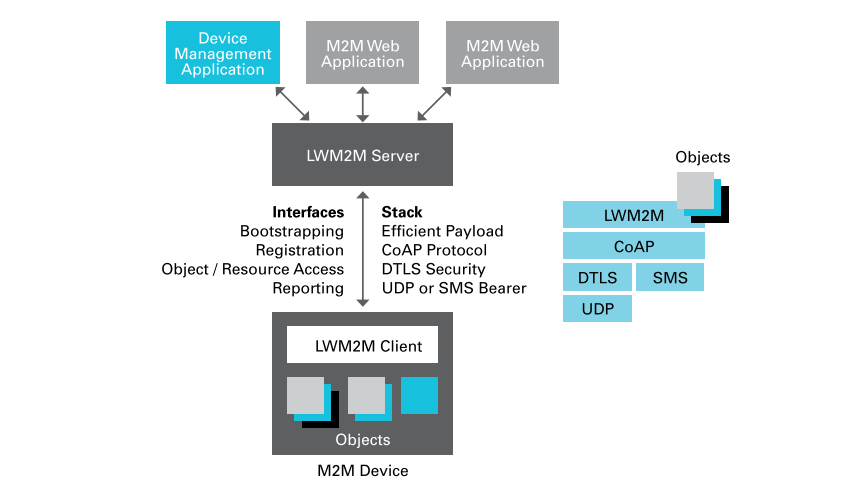
\includegraphics[width=\textwidth]{images/LWM2M-Architecture}
		\caption{LWM2M Architecture}
		\label{fig:LWM2MArchitecture}
	\end{center}
\end{figure}

The LWM2M Enabler defines the application layer communication protocol between Server and Client. It is separated into four logical interfaces, namely, Bootstrap, Device Discovery and Registration, Device Management and Service Enablement, and Information Reporting. Diagram showing interfaces and corresponding messages is illustrated in ~\ref{fig:LWM2MInterfaces}.

\begin{enumerate}
	\setlength{\itemsep}{1pt}
	\item Bootstrap: allows LWM2M Bootstrap server to manage keying, access control and to configure device for communication with the Server.
	\item Device Discovery and Registration: allows Server to discover devices and register their capabilities, e.g., which objects and how to access them does a device have.
	\item Device Management and Service Enablement: allows LWM2M Server to manage devices and provide M2M service by sending operations to devices and getting corresponding responses from them.
	\item Information Reporting: This is a core interface in LWM2M, which allows reporting of resource information. It can be triggered periodically, on events or on request.
\end{enumerate}

Communication model of LWM2M is based on CoAP methods similar to HTTP verbs GET, POST, PUT, DELETE to manipulate \emph{resources} on devices. Compared to HTTP, CoAP starts with only four bytes of overhead in binary encoded message and is easily translatable to HTTP. Unlike HTTP, CoAP messages are exchanged asynchronously between CoAP end-points over a datagram-oriented transport, in this case UDP.

In LWM2M Enabler, each individually addressable piece of information is called a Resource and groups of Resources are logically organized into Objects. For example, predefined object \emph{Location} contains all resources needed for locating the device. Full list of existing objects can be found at OMA registry \footnote{http://www.openmobilealliance.org/wp/OMNA/LwM2M/LwM2MRegistry.html}.

\begin{figure}[ht]
	\begin{center}
		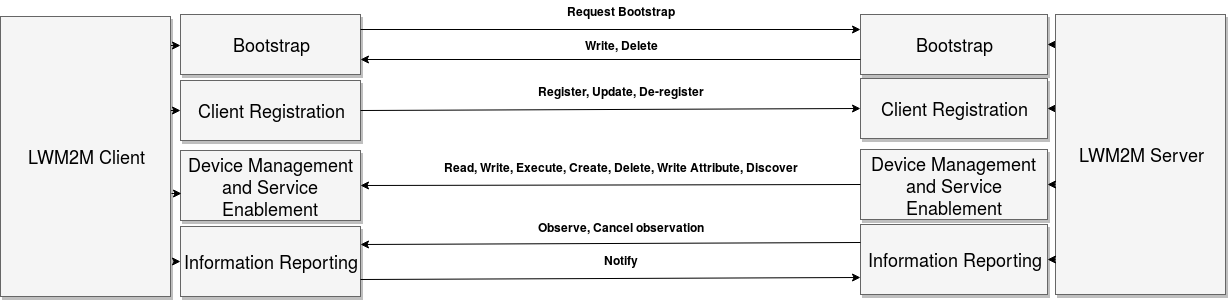
\includegraphics[width=\textwidth]{images/LWM2M-Interfaces}
		\caption{LWM2M Interfaces}
		\label{fig:LWM2MInterfaces}
	\end{center}
\end{figure}

\subsection{World-wide-web Consortium (W3C) - Web Of Things (WOT)}

Since there are many IOT platforms already existing, it is becoming a big problem for developers creating applications that span them. The solution W3C proposes aims to enable worldwide discovery and interoperability by exposing these platforms through the Web with a new class of webservers that support an open framework for the WOT as pictured on ~\ref{fig:WOTWebservers}. In other words, WOT aims to interconnect existing IOT platforms and complement available standards, to reduce cost and risk, and to boost market opportunities.

\begin{figure}[ht]
	\begin{center}
		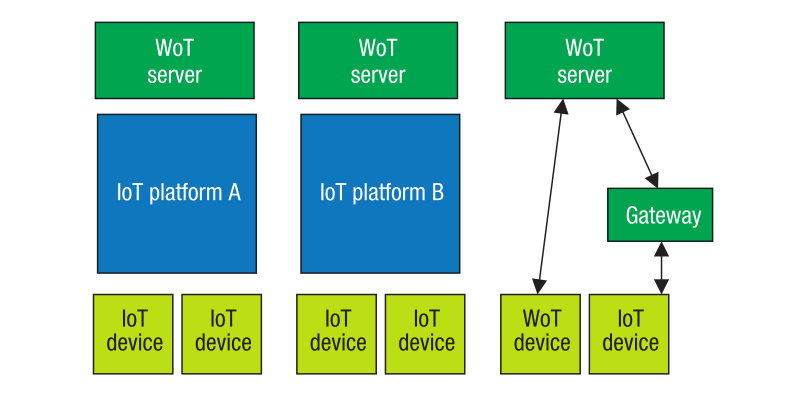
\includegraphics[width=\textwidth]{images/WOTWebservers}
		\caption{WOT framework that bridges the multiple existing IOT platforms}
		\label{fig:WOTWebservers}
	\end{center}
\end{figure}

In W3C WOT all things (devices) are modeled as events, properties and actions, while also possessing metadata describing location of the device, serial number and similar. Firstly, events represent notifications from device to server, such as "battery low" or "the door just opened". Secondly, properties represent information that can be checked through server, such as the temperature or the state of the light switch (on or off). Finally, actions represent commands to coming from server to the device, such as "move the crane from position x to position y" or "turn off". In order to retrieve matadata for things, WOT uses JavaScript Object Notation for Linked Data (JSON-LD).

Analogous to the role played by the Internet as an abstraction layer for networks and networking technologies, WOT describes an abstraction layer over heterogeneous IOT standards, communication patterns, protocols and data formats. This abstraction layer is pictured on figure ~\ref{fig:WOT}, where applications interact with software objects for things (devices, either virtual or physical). Webservers providing this abstraction can be placed on the edge of the network (or in the fog or cloud) to provide efficiency.

\begin{figure}[ht]
	\begin{center}
		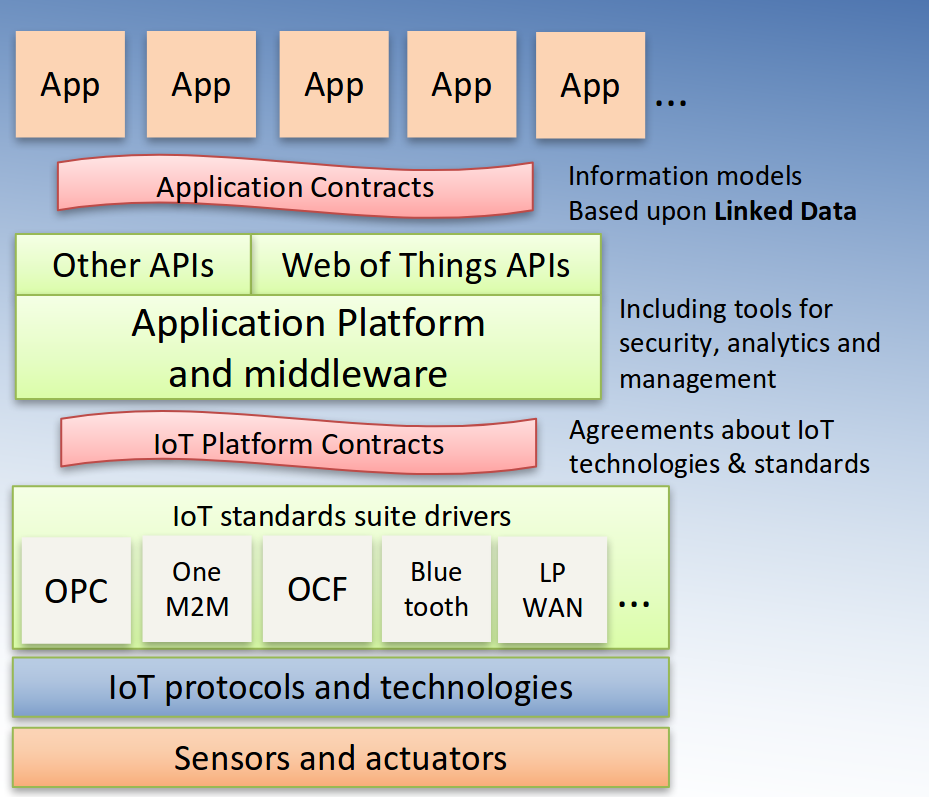
\includegraphics[width=\textwidth]{images/WOT}
		\caption{WOT abstraction layer}
		\label{fig:WOT}
	\end{center}
\end{figure}

Regarding security, WOT is building upon existing security standards such as IOT security foundation, and IOT platforms such as oneM2M (described in section ~\ref{section:Standardization}), claiming to provide end to end security. 

W3C WOT is a new standard, with the working group formed in the beginning of 2017. Since it is a new standard, their work has mostly been abstract, without any real implementations. It is relatively heavy weight compared to LWM2M standard, and focuses on providing a bridge between different platforms unlike LWM2M, that proposes a new solution not necessarily compatible with other existing solutions. Because the work on WOT is in a very early phase and reasons described above I have chosen to make use of LWM2M standard for this thesis.

\section{Policy Based Communications for 5G Mobile with Customer Edge Switching}
\label{CES}

Particularly interesting work by \cite{Kantola} proposes a policy based communication with built in security, while also addressing classical weaknesses of Internet, namely, address spoofing, unwanted traffic and DoS attacks. It is based on a principle that before establishing communication between two hosts (or networks) they need to negotiate interests, and only if they are matching communication is established. These interests are described with a policy.

This work proposes to replace Network Address Translator (NAT) from the edge of the network with their own Customer Edge Switch (CES) node. This node will act exactly like NAT if the sender, who is behind a CES node, is interacting with a receiver using legacy ip. On the other hand, if the situation is reversed CES node will act as a \emph{realm gateway}. Only if both actors are behind CES node it will act as a cooperative firewall negotiating interests of sender and receiver. Because of this, CES can be applied one network at a time making it suitable for IIOT purposes, where vertical fragmentation is a big issue.

Furthermore, CES allows efficient communication by dropping unwanted traffic at the edge and in that way reducing amount of traffic that passes trough network. Also, CES makes use of Domain Name Servers (DNS) to find receivers faster using Fully Qualified Domain Names (FQDN) and MS-ISDN numbers.

In essence, policy database holds all policies and can be accessed through API. Before communication is established, policies of both actors are checked and if they match communication is allowed. Example is shown on ~\ref{fig:PolicyBasedCommunicationExample}.

\begin{figure}[ht]
	\begin{center}
		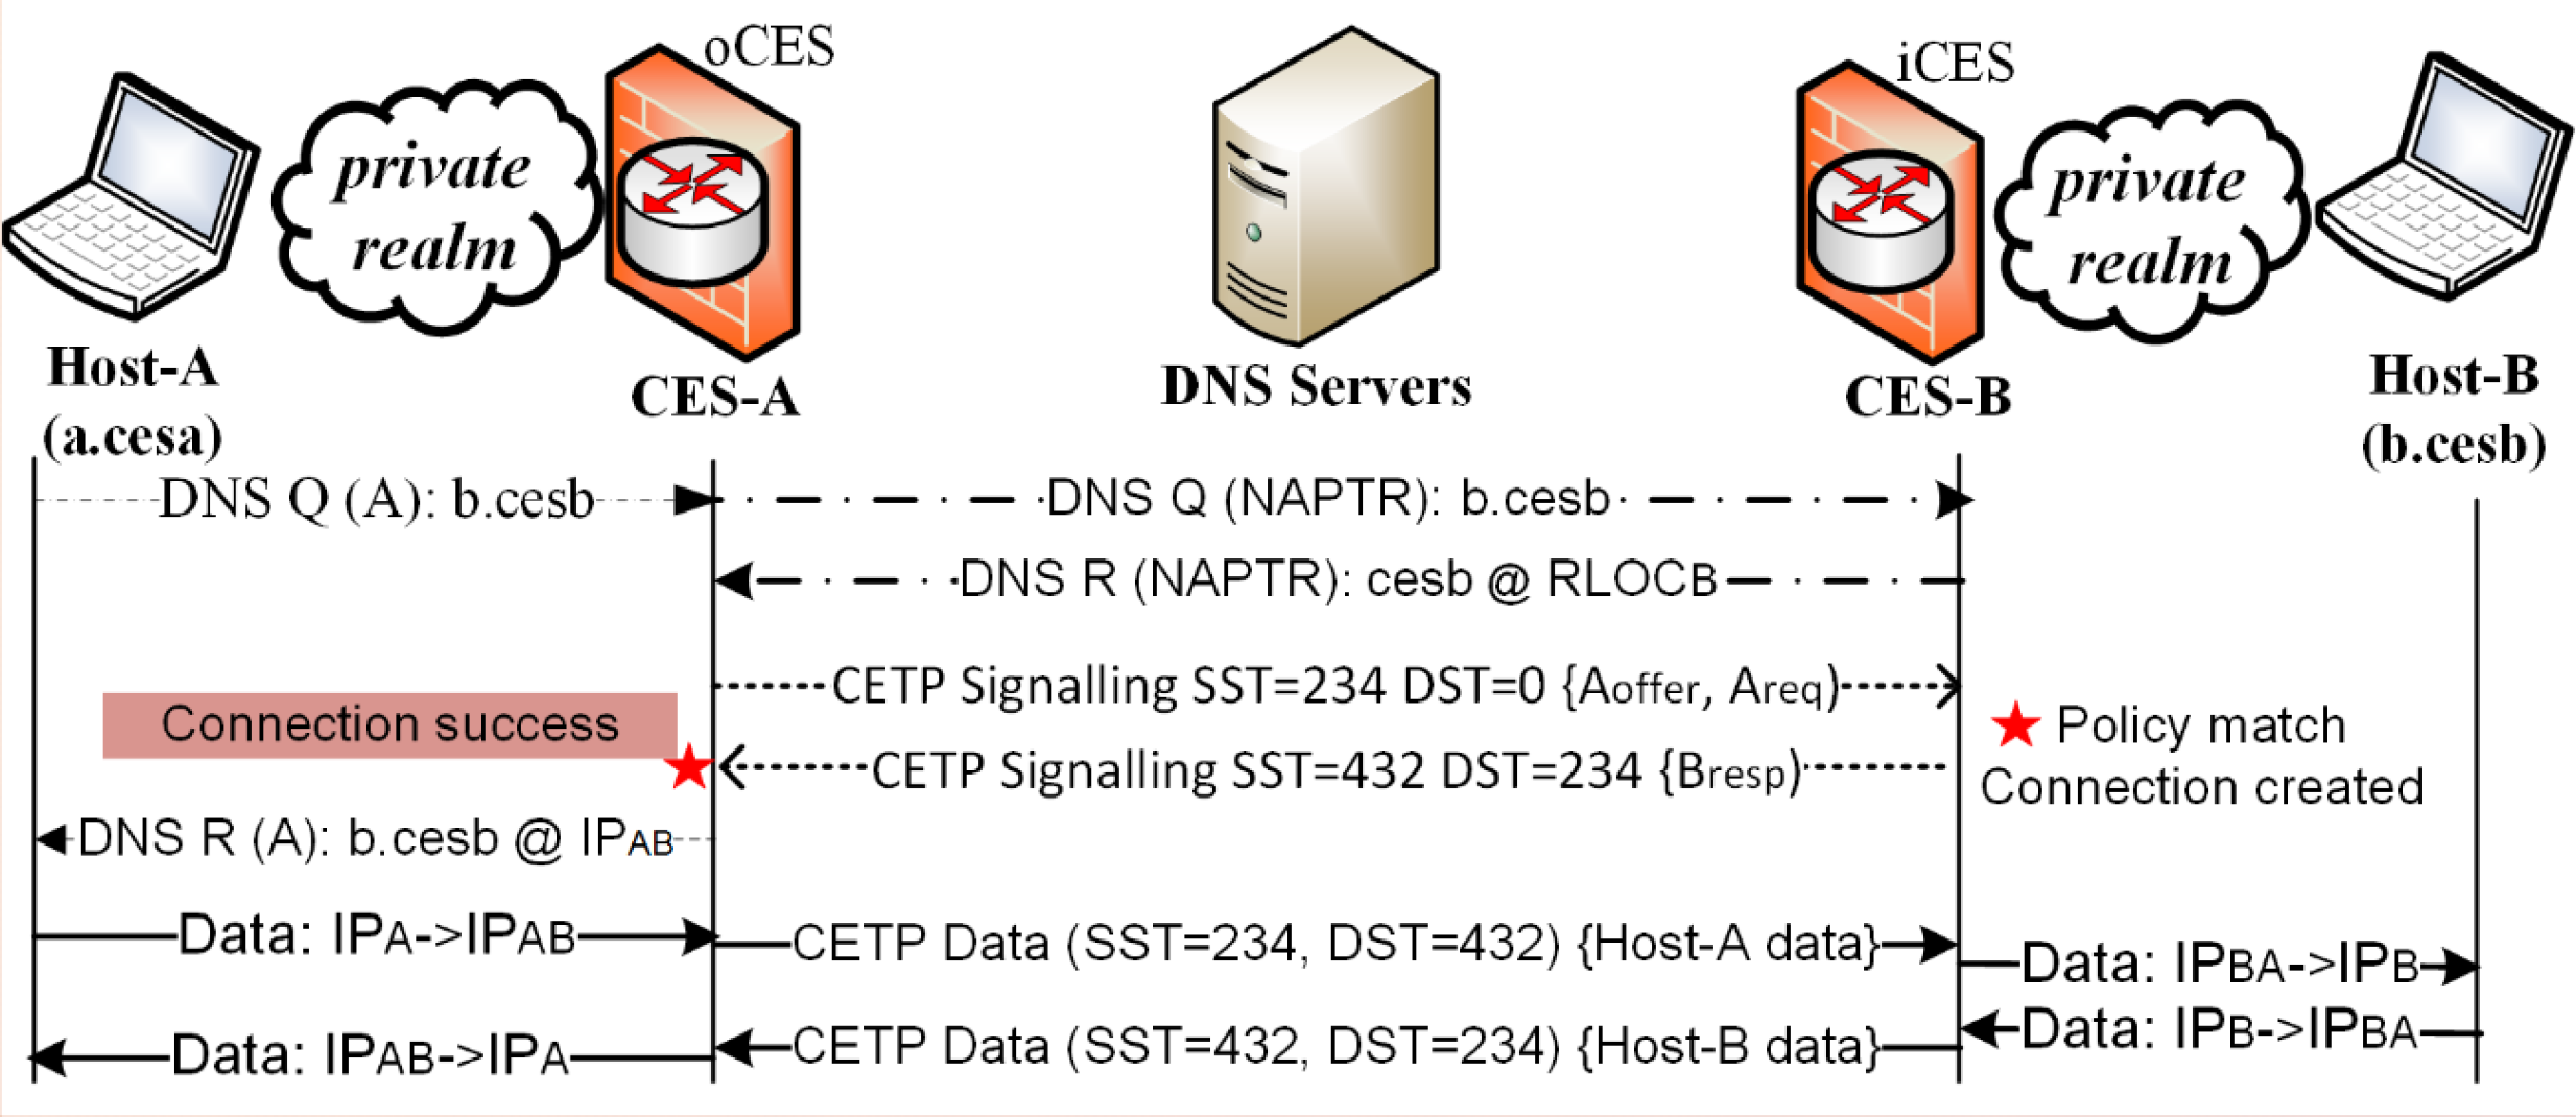
\includegraphics[width=\textwidth]{images/PolicyBasedCommunicationExample}
		\caption{CES communication example}
		\label{fig:PolicyBasedCommunicationExample}
	\end{center}
\end{figure}
